\documentclass{cnriut} % Ne pas modifier
\annee{2025}           % Ne pas modifier
\lieu{Bayonne} % Ne pas modifier

\usepackage{graphicx}  % inclusion de graphiques
\usepackage[url=false,urldate=none]{biblatex}
\addbibresource{references.bib}
\usepackage{tabularx}

\titre{Développement d'un framework de suivi et d'évaluation de l'impact à travers un data warehouse sémantique pour les méta-organisations}

% \auteurs{%
%   Clément Combier$^{1,*}$ \and
%   Adel Noureddine$^2$ \and
%   Jose Enrique Armendariz-Inigo$^3$ \and
%   Philippe Arnould $^2$
%   }

% \courriels{%
%   clement.combier@univ-pau.fr \and
%   adel.noureddine@univ-pau.fr    \and
%   enrique.armendariz@unavarra.es \and
%   philippe.arnould@univ-pau.fr
% }


\affiliations{%
  $^1$ Université de Pau et des Pays de l'Adour \\
   E2S-UPPA, LIUPPA, Mont de Marsan, France \\
  \\
  $^2$ IUT de Pays de l'Adour \\
  E2S-UPPA, LIUPPA, Pau, France\\
  \\
   $^3$ Universidad Pública de Navarra \\
  Pampelune, Espagne\\
  \\
  $^4$ IUT de Pays de l'Adour \\
  E2S-UPPA, LIUPPA, Mont de Marsan, France\\
}

\correspondingauthors{Le/les auteur(s) avec la marque * sont auteur(s) correspondant(s).}

\themes{%
 Gestion - Informatique - Communication 
}

\resume{Ce travail de recherche vise à développer un cadre pour les méta-organisations (notamment les alliances d'universités européennes) pour surveiller et évaluer leur impact sur la société en utilisant des solutions données. Les alliances d'universités européennes, telles que celles créées dans le cadre de l'initiative européenne des universités, nécessitent des outils et des méthodologies spécifiques pour évaluer leur impact, qui dépasse celui des organisations individuelles. Ce cadre devra prendre en compte la complexité des organisations interconnectées et la nécessité de flexibilité pour répondre aux besoins spécifiques de chaque organisation membre.}

\motscles{data warehouse, web sémantique, méta-organisation, mesure d'impact}

\sectionsCNU{27}

%CONSERVER LA VALEUR "OUI" OU "NON" si l'article sera présenté par un doctorant durant le CNRIUT'2025.
\doctorant{OUI}


\begin{document}
\creationEnTete        % Ne pas modifier

\section{Introduction}
La globalisation et l'internationalisation de l'éducation ont connu une accélération spectaculaire ces dernières années, en particulier au sein des établissements d'enseignement supérieur. Ce mouvement mondial s'est popularisé en Europe grâce à l'initiative Erasmus+ des universités européennes. En 2019, l'initiative des universités européennes (EUI) a été lancée avec pour mission de promouvoir, de faciliter et de diffuser la nécessité d'alliances interuniversitaires en Europe. Depuis, 64 alliances, couvrant plus de 35 pays, regroupant plus de 500 universités, ont été créées. Ces alliances entraînent des changements et des transformations importantes, apportant de nouveaux besoins et défis. Pour assurer le développement et la durabilité des universités européennes à venir, il est nécessaire de surveiller et d'évaluer l'impact lié à la vision à long terme de ces alliances.

Les alliances européennes pourraient être caractérisées en suivant le modèle proposé en 2005 par G. Ahrne et N. Brunsson \cite{ahrne_organizations_2005}, en appliquant le concept de méta-organisations pour désigner le regroupement de nombreuses organisations autour d'objectifs et de projets communs. 

De nombreux frameworks et méthodologies ont été développés et proposés au fil des ans sur la théorie des changements et  d'évaluation de l'impact. Cependant, ces cadres peuvent ne pas fournir aux méta-organisations les outils et la flexibilité des organisations simples. Ceci prouve l'importance d'une méthodologie plus large pour les méta-organisations, tout en gardant une ancre pour chaque organisation partenaire.

Ce projet de recherche vise à développer un cadre pour les méta-organisations (dans ce contexte, les alliances d'universités européennes) pour surveiller et évaluer leur impact sur la société en utilisant des solutions orientées données.

\section{État de l'art}
Les alliances universitaires ont attiré l'attention, notamment depuis le lancement en 2019 de l'Initiative des universités européennes (IUE). À mesure que les alliances s'étendent, il est nécessaire d'évaluer leur impact sociétal et de développer des stratégies de suivi. Cet examen décrit la recherche sur la mesure de l'impact, la Théorie du Changement (TdC) et les systèmes de Suivi et d'Évaluation (S\&E) au sein de méta-organisations comme les alliances universitaires. En explorant ces sujets, nous visons à construire un cadre pour évaluer leur impact. Nous définirons d'abord les concepts clés de notre étude.

\subsection{Impact}
L'impact désigne généralement les effets à long terme des activités sur leur environnement. Nous retenons la définition du Comité d'Aide au Développement (CAD) de l'Organisation de Coopération et de Développement Économiques (OCDE) : "effets à long terme positifs et négatifs, primaires et secondaires, produits par une intervention de développement, directement ou indirectement, intentionnels ou non" \cite{oecd_quality_2010}.

L'identification d'indicateurs pertinents reste un défi. La Figure \ref{fig:simplified-impact-chain} illustre une chaîne d'impact simplifiée reliant ressources, activités, résultats et effets \cite{peersman_when_2016}.

\begin{figure}
    \centering 
    
\includegraphics[width=1\linewidth]{images/Diagrams-IMPACT.png} 
    \caption{Chaîne d'impact simplifiée\cite{peersman_when_2016}}
    \label{fig:simplified-impact-chain} 
\end{figure}

\subsection{Théorie du changement}
La théorie du changement a évolué au fil du temps, passant de la "Théorie des trois étapes du changement" de Kurt Lewin\cite{lewin_frontiers_1947} aux modèles élargis et cycliques proposés par Lippitt et al.\cite{lippitt_dynamics_1958} et Prochaska et DiClemente\cite{prochaska_stages_1983}. Ces théories, comme la Théorie de l’action raisonnée et du comportement planifié, introduisent des concepts clés tels que le "contrôle perçu", mais manquent d’une perspective sociétale. 

Nous explorons la TDC de la Littératie Politique, qui combine une approche politiquement informée et stratégique, essentielle pour la planification, le suivi et l'évaluation des changements au sein des méta-organisations.

\subsection{Système de Suivi et d’Évaluation}
Les systèmes de Suivi et d’Évaluation (S\&E) combinent une évaluation régulière pour quantifier les mesures et un suivi continu pour détecter les anomalies, garantissant ainsi des données fiables tout au long du cycle de vie d’un projet.

\subsection{Data warehouse et base de connaissances partagée}
Les entrepôts de données orientés connaissances permettent de centraliser et d’exploiter des informations souvent abstraites, comme l’impact sociétal. Ils offrent une vision commune à travers l’alliance, facilitant une évaluation précise via des indicateurs statistiques.


\section{Notre approche}
\begin{figure}
    \centering
    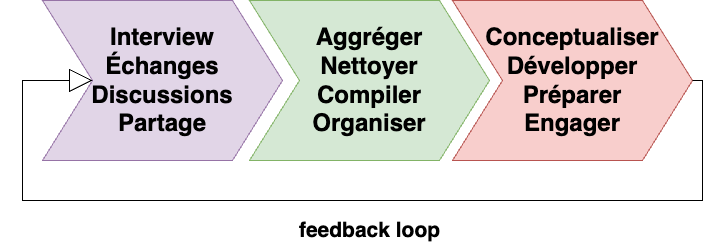
\includegraphics[width=0.75\linewidth]{images/Diagrams-Simplified framework chain Our approach.png}
    \caption{Notre approche simplifié}
    \label{fig:simplified-approach}
\end{figure}
Notre approche propose un cadre multi-axes pour aider les méta-organisations à évaluer l'impact via des méthodologies et outils basés sur les données. Nous présentons un cadre multi-étapes pour construire une solution de stockage de données orientée impact, allant de la collecte de preuves à l'analyse des indicateurs par des entretiens axés sur l'impact. Ce système permettrait aux méta-organisations de surveiller et d'évaluer régulièrement leur impact tout en engageant efficacement les partenaires internes et externes dans les changements. Nous avons identifié trois activités essentielles : la discussion, l'évaluation et la construction du système. Notre travail vise à transformer positivement le changement à l'intérieur des organisations et méta-organisations, avec des actions planifiées pour gérer la résistance et soutenir le changement via des feedbacks positifs. 

\section{Résultats}
Lors de cette première année, nous avons mis en œuvre une méthodologie structurée pour collecter les indicateurs et les besoins spécifiques des différentes tâches de l’alliance UNITA. À partir d'entretiens collaboratifs, nous avons récupéré une liste d’indicateurs clés, validés en partenariat avec chaque équipe.

Ce processus est en cours de finalisation grâce à une deuxième série d’interviews dédiée à la validation des données. Parmi les 150 indicateurs d’outputs et 75 indicateurs d’outcomes identifiés, chacun doit être validé par les parties prenantes avant son intégration complète dans le data warehouse (DWH).

Une fois les données nettoyées pour éliminer incohérences et doublons, elles seront intégrées dans le DWH centralisé de l’alliance UNITA. Ce système facilite le suivi des progrès, l’identification des tendances, et la prise de décisions stratégiques. Lorsqu’un indicateur est validé pour une tâche, le DWH est configuré pour permettre la collecte des données auprès des institutions membres. Cela amorce les travaux d’analyse, notamment la création de rapports et la prédiction de l’impact.

La saisie et l’intégration des données se font de manière semi-automatique via des formulaires standardisés. Les institutions partenaires remplissent ces formulaires pour transmettre les données de leurs universités, qui sont ensuite enregistrées directement dans le DWH. Ces informations sont transformées pour alimenter UNITApedia, une solution MediaWiki sémantique connectée au DWH. Cet outil fournit des rapports interactifs et un accès transparent aux données pour tous les acteurs impliqués.

La Table~\ref{tab:indic_ex} illustre une sélection d’indicateurs pertinents utilisés pour mesurer les résultats (outputs) et les effets (outcomes) des activités de l’alliance UNITA.

\begin{table}[h]
    \caption{Exemples d’indicateurs outputs (sélection)}
    \centering
    \begin{tabular}{|l|l|}
        \hline
        \textbf{Indicateurs} & \textbf{Unités} \\ \hline
        Pourcentage de projets UNITA évalués & \% \\ \hline
        Nombre d’événements de matchmaking & Nombre \\ \hline
        Nombre de publications scientifiques & Nombre \\ \hline
    \end{tabular}
    \label{tab:indic_ex}
\end{table}


\section{Remerciements}
Je souhaiterais remercier l'alliance UNITA pour son aide sur ce travail ainsi que sa participation comme modèle de base pour explorer ses possibilités et permettre d'améliorer les alliances universitaires de demain.

\printbibliography


\end{document}

